% pLaTeX でタイプセットする
% platex masterabs && biber masterabs && platex masterabs && platex masterabs && dvipdfmx masterabs.dvi

%%%%%%%%%%%%%%%%%%%%%%%%%%%%%%%%%%%%%%%%%%%%%%%%%%%%%%%%%%%%%%%%
%%%%%%%  Example: extended abstract for master thesis
%%%%%%%  version 1.0
%%%%%%%  file name: template.tex
%%%%%%%%%%%%%%%%%%%%%%%%%%%%%%%%%%%%%%%%%%%%%%%%%%%%%%%%%%%%%%%%
%--------------- start preamble -------------------------------
\documentclass[a4paper]{jarticle} % 10pt fonts, default fonts
%\documentclass[a4paper,11pt]{jarticle} % 11pt fonts
%\documentclass[a4paper,12pt]{jarticle} % 12pt fonts
%--------------------------------------------------------------
\usepackage{masterabs} % 修士論文アブストラクトのスタイルファイル
%--------------------------------------------------------------
\usepackage{amsmath,amsthm,mathrsfs} % amslatex モードの指定
\usepackage{amsfonts,amssymb,txfonts} % amsfonts の指定
\usepackage[dvipdfmx]{graphicx} % 図の挿入の指定 (\includegraphicsなど)
%--------------------------------------------------------------
\columnseprule = 0.4pt % two columnの真ん中に縦線を引く
%--------   英文の場合: 表,図、参考文献を英語に変更 ----------------
\initenglish % 本文が英文の場合は % を取る(表=>Tab., 図=>Fig.など)
%--------------------------------------------------------------------
%

\theoremstyle{definition}
\newtheorem{thm}{Theorem}[section]
\newtheorem{dfn}[thm]{Definition}
\newtheorem{eg}[thm]{Example}
\newtheorem{lem}[thm]{Lemma}
\newtheorem{prop}[thm]{Proposition}
\newtheorem{cor}[thm]{Corollary}
\theoremstyle{remark}
\newtheorem{rem}[thm]{Remark}

\DeclareMathOperator{\rank}{rank}
\DeclareMathOperator{\NS}{NS}
\DeclareMathOperator{\Tr}{Tr}
\DeclareMathOperator{\chara}{char}
\DeclareMathOperator{\Spec}{Spec}
\DeclareMathOperator{\ch}{ch}
\newcommand{\Neron}{N\'eron}

\usepackage[T1]{fontenc}

% \usepackage[sorting=nyt,date=year,isbn=false,doi=false,url=false,giveninits]{biblatex} % biblatexを使用するためのパッケージ
\usepackage[backend=biber, bibstyle=math-numeric,sentencedtitle=false, dashed=false]{biblatex}
\renewbibmacro*{in:}{} % in: を削除
\DeclareFieldFormat[book]{title}{\textit{#1}} % book の title を bold にしない
\DeclareFieldFormat[article,misc]{title}{\textup{#1}} % article の title を italic にしない
\addbibresource{references.bib}

%-------------- end preamble ----------------------------------
%
%%%%%%    TEXT START    %%%%%%

\begin{document}
%
%-------------- two column -------------------------
\twocolumn[ % two column の場合は,先頭の % を取る
%---------------------------------------------------
%
%---------------------------------------------------------------------------
\no_tlfnmark % タイトルの最後にfootnote markを付けない場合は,先頭の % を取る
%---------------------------------------------------------------------------
%%% タイトルが 1行 \title{タイトル}を使う
%%% タイトルが 2 行にわたるときは \2ltitle{1行目}{2行目}を使う
%---------------------------------------------------------------
% \title{On the Mordell-Weil groups of elliptic surfaces associated with Frey curves of degree two} % 1 行用
%
\2ltitle{On the Mordell-Weil groups of elliptic surfaces}{associated with Frey curves of degree two} % 2 行用
%
%-------------------------------------------
% 日本語指導教員,著者名など
%-------------------------------------------
\begin{preliminary}
\profname{栗原将人教授}       %% 指導教員の名前 + 講師,准教授,教授
\name{82313206}{八木颯仁} %% 学籍番号, 著者名
\end{preliminary}
%
%---------- two column ----------------------
]% two columnの場合は,先頭の % を取る
%--------------------------------------------
%
%------- footnote に英文のタイトルを記述したいとき ----------------
% \etitle{On the Mordell-Weil groups of elliptic surfaces associated with Frey curves of degree two}
%----------------------------------------------------------------
%
\init_fnmark % 脚注マークの初期化(アラビア数字に変更)
%%%%%%%%%%%%%%%%%%%%%%%%%%%%  本文 %%%%%%%%%%%%%%%%%%%%%%%%%%%%%

\section{Introduction}
An elliptic curve defined over a field $K$ of characteristic $\neq 2$ is a curve defined by a Weierstrass equation
\begin{equation*}
    E: y^{2} = x^{3} + Ax^2 + Bx + C
\end{equation*}
where $A,B,C \in K$ and the discriminant $\Delta = -4A^3C + A^2B^2 + 18ABC - 4B^3 - 27C^2$ is nonzero.
When $K=\mathbb{Q}$, we can define an addition law geometrically on points on an elliptic curve defined over $\mathbb{Q}$.
%  as shown in Figure~\ref{fig:elliptic_curve}.
For two points $P,Q$ on $E$, the point $-(P+Q)$ is defined as the third point of intersection of the line passing through $P$ and $Q$ with the curve.
The sum $P+Q$ is the point symmetric to $-(P+Q)$ with respect to the $x$-axis.
The definition can be extended to any field $K$ of characteristic $\neq 2$.
The set of points on an elliptic curve forms an abelian group with the identity element being the point at infinity.
The Mordell-Weil group $E(K)$ is a group consisting of all $K$-rational points on $E$.
The Mordell-Weil theorem states that the Mordell-Weil group is a finitely generated abelian group if $K$ satisfies some finite conditions.
The Mordell-Weil group is an important object in the study of the arithmetic of elliptic curves.
Especially, the rank of the Mordell-Weil group is important and difficult to determine, in general.
% \begin{figure}[ht]
%     \centering
%     \caption{$E: y^2 = x(x-3^2)(x+4^2)$}
%     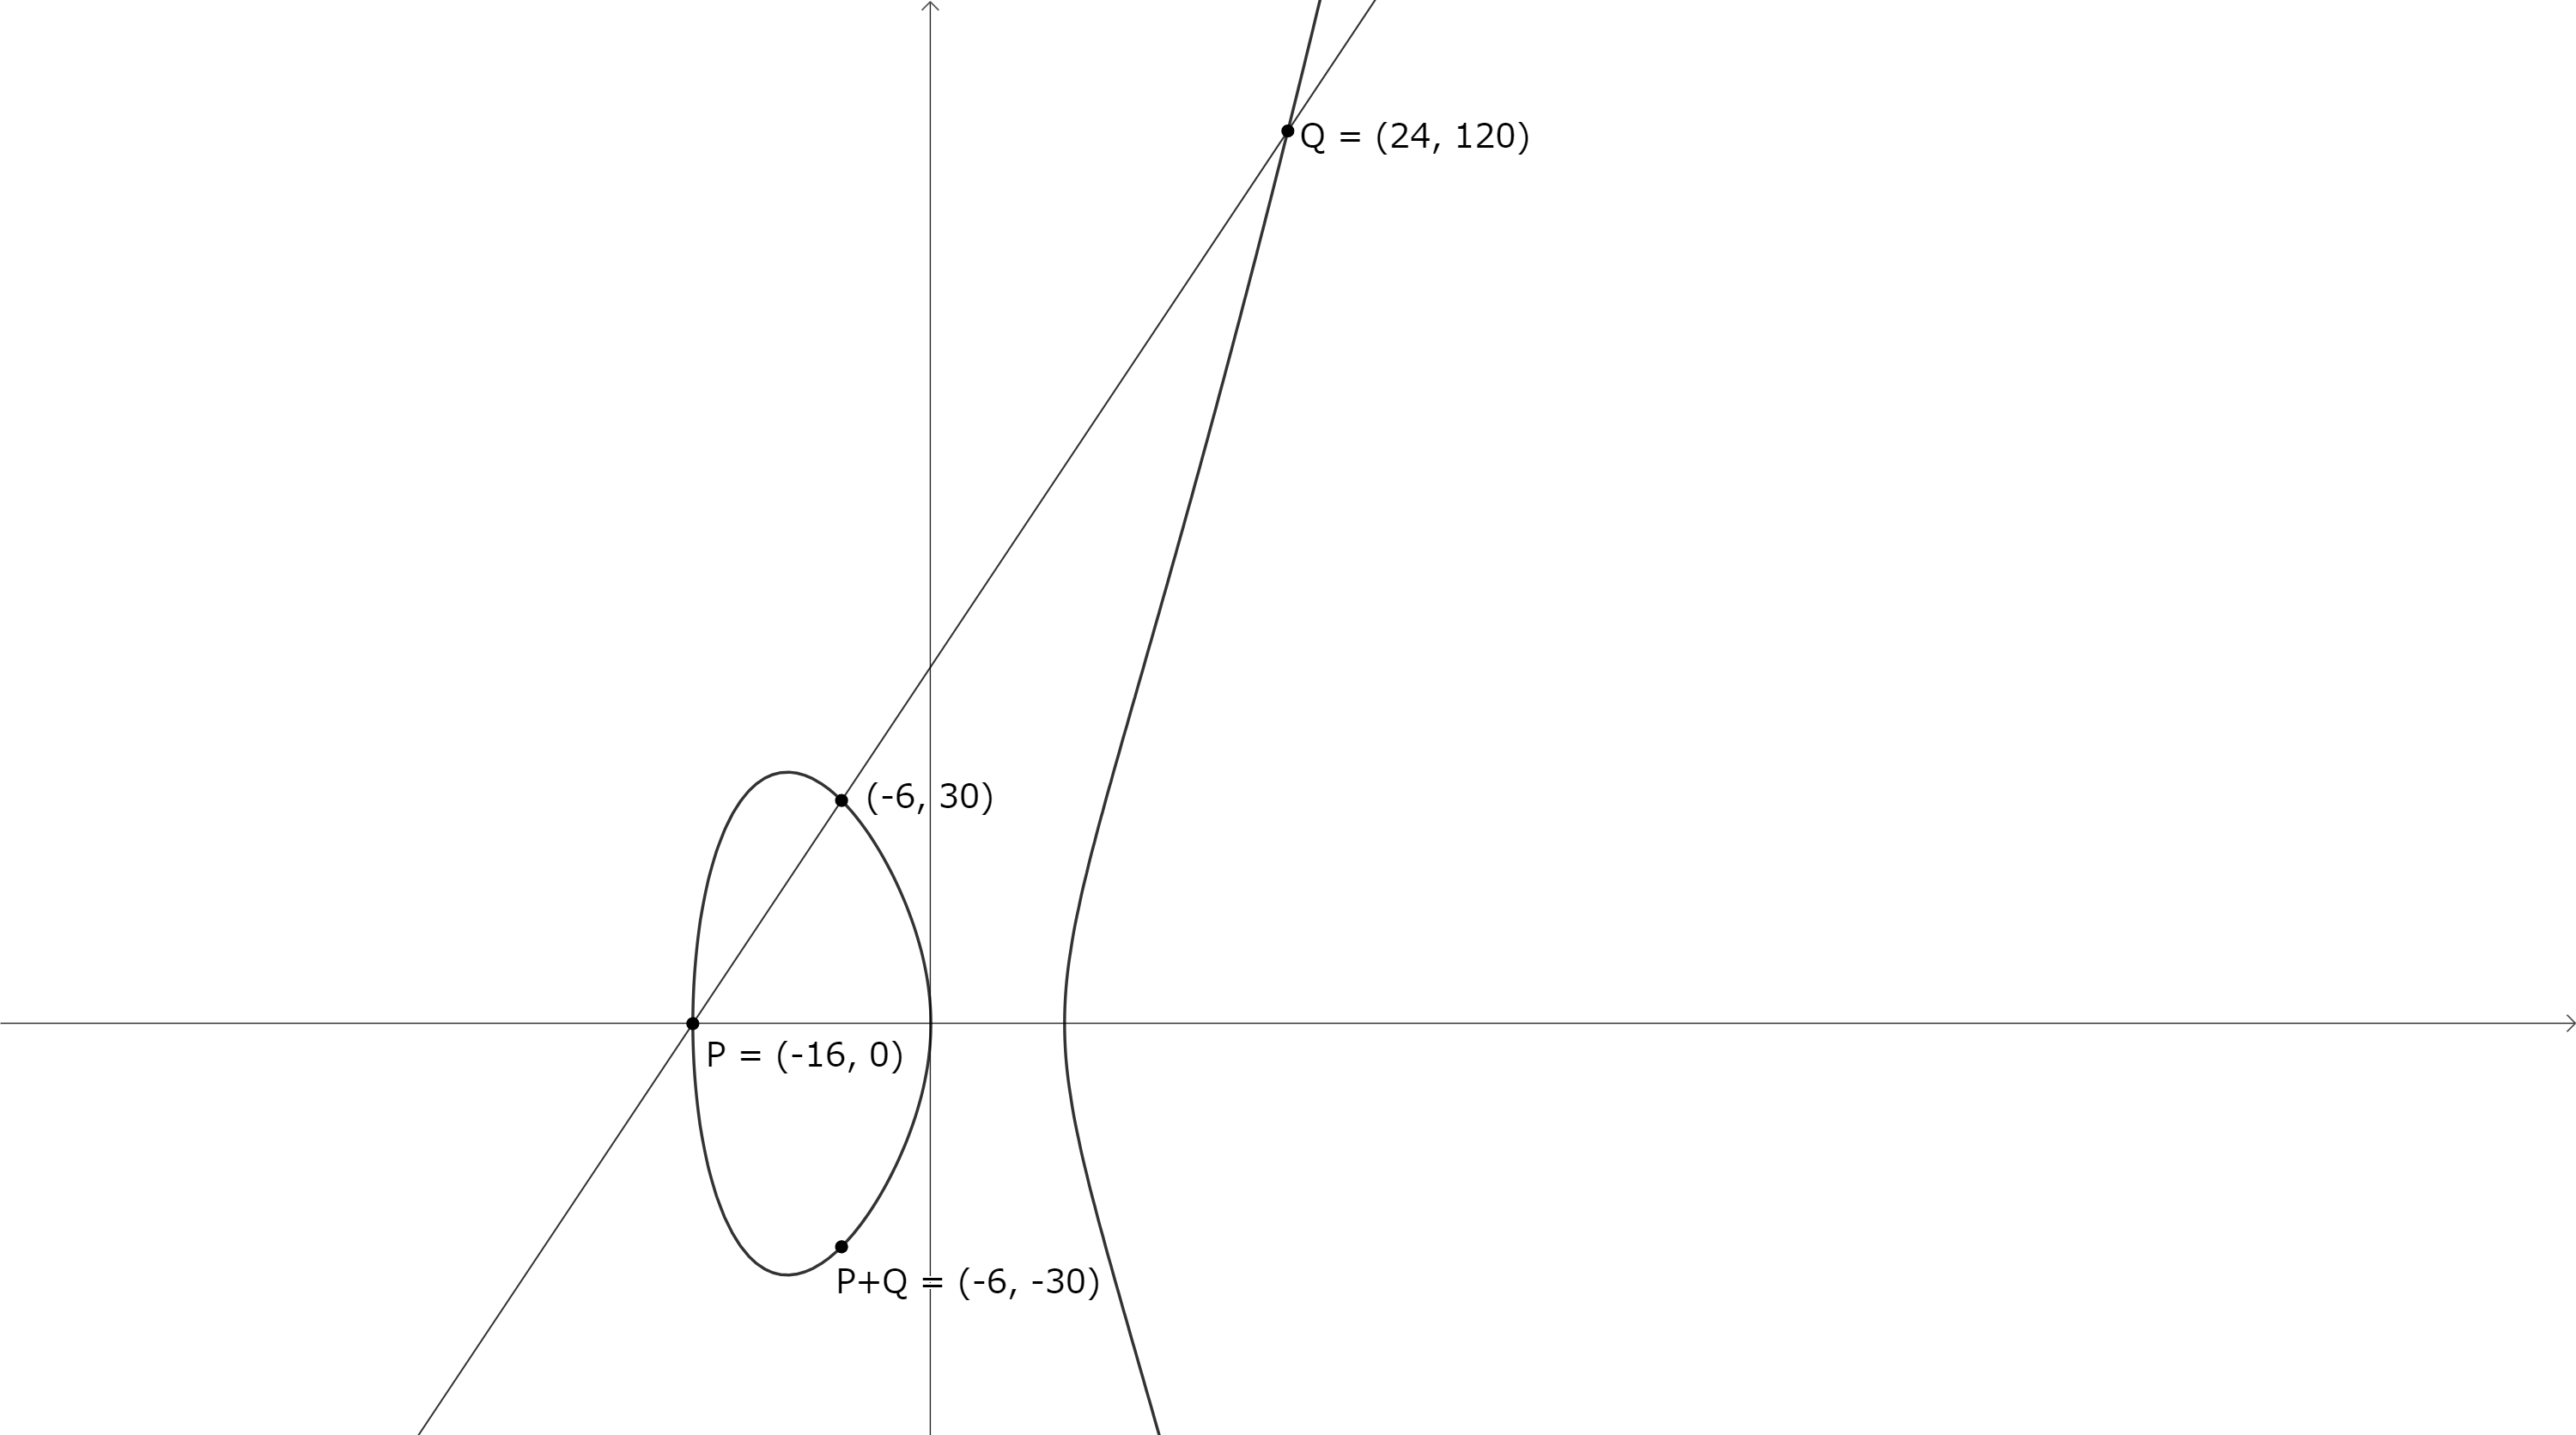
\includegraphics[keepaspectratio, width=0.6\linewidth]{figures/3-4-5.png}
%     \label{fig:elliptic_curve}
% \end{figure}

Let $(a,b,c) \in \mathbb{Z}^3$ be a Pythagorean triple, namely integers satisfies $a^{2} + b^{2} = c^{2}$, and consider the elliptic curve defined by the Weierstrass equation
\begin{equation}
    \label{eq:2frey}
    y^{2} = x(x - a^{2})(x + b^{2}).
\end{equation}
This is the case $n=2$ of the Frey curve.

We can parameterize Pythagorean triples $(a,b,c)$ by $m,n \in \mathbb{Z}$ with $(m,n)=1$ as $(a,b,c) = (2mn, m^{2} - n^{2}, m^{2} + n^{2})$.
Then the equation \eqref{eq:2frey} can be written as $y^{2} = x(x - 4m^2n^2)(x + (m^{2} - n^2)^{2})$.
We replace $x,y$ by $n^2x, n^3y$ and put $s = m/n$.
Then we get an elliptic curve
\begin{equation*}
    \label{eq:E_{1,s}}
    E_{1,s}: y^{2} = x(x - 4s^{2})(x + (s^{2} - 1)^{2}).
\end{equation*}
We consider $E_{1,s}$ as an elliptic curve over a function field $\overline{\mathbb{Q}}(s)$, where $\overline{\mathbb{Q}}$ is the algebraic closure of $\mathbb{Q}$.
We associate an elliptic surface $\mathcal{E}_{1,s} \to \mathbb{P}^1$ to $E_{1,s}$.


\section{Main Theorem}

\begin{prop}
    \label{thm:E_{1,s}}
    The Mordell-Weil group of $E_{1,s}$ over $\overline{\mathbb{Q}}(s)$ satisfies
    \begin{equation*}
        E_{1,s}(\overline{\mathbb{Q}}(s)) \cong \mathbb{Z} / 4 \mathbb{Z} \oplus \mathbb{Z} / 4 \mathbb{Z},
    \end{equation*}
    especially the rank is $0$.
    The torsion subgroup is generated by
    \begin{align*}
        T_1 & := (2s(s+1)^2, 2s(s+1)^2(s^2+1)),                               \\
        T_2 & := (2 \sqrt{-1} s(s^2-1),2 \sqrt{-1} s(s+\sqrt{-1})^2(s^2-1)).
    \end{align*}
\end{prop}
\vspace{1em}

By substituting $s = \frac{2t}{t^{2} - 3}$ into $E_{1,s}$, we get a new family of elliptic curves
\begin{equation*}
    E_{2,t}: y^{2} = x \left(x - 4 \left(\frac{2t}{t^{2} - 3} \right)^{2} \right) \left(x + \left(\left(\frac{2t}{t^{2} - 3} \right)^{2} - 1 \right)^{2} \right),
\end{equation*}
which is a subfamily of $E_{1,s}$.
The following is our main result.
\begin{thm}
    \label{thm:E_{2,t}}
    The Mordell-Weil group of $E_{2,t}$ over $\overline{\mathbb{Q}}(t)$ satisfies
    \begin{equation*}
        E_{2,t}(\overline{\mathbb{Q}}(t)) \cong \mathbb{Z} \oplus \mathbb{Z} / 4 \mathbb{Z} \oplus \mathbb{Z} / 4 \mathbb{Z},
    \end{equation*}
    especially the rank is $1$.
    The torsion subgroup is generated by $T_1$ and $T_2$ in Theorem~\ref{thm:E_{1,s}} with $s = \frac{2t}{t^{2} - 3}$.
\end{thm}
The important point is that we prove that the generic rank of $E_{2,t}$ is exactly $1$, not only the existence of a point of infinite order.
Our proof is based on the method of Naskręcki in \cite{ref:naskrecki2013}.

\section{Sketch of the proof}
The torsion subgroup is relatively simple, so only rank is discussed here.
The proof is divided into two major steps.
First, we relate the Mordell-Weil rank to the Picard number, and then the Picard number is evaluated.
The following theorem plays a key role in the first step.
\begin{thm}{(Shioda-Tate formula, \cite[Corollary 5.3]{ref:shioda1990})}
    \label{thm:shioda}
    Let $\mathcal{E} \to C$ be an elliptic surface over a smooth projective curve $C$ over an algebraically closed field $k$.
    Let $R \subset C$ be the set of points where the special fiber of $\mathcal{E}$ is singular.
    For each $v \in R$, let $m_{v}$ be the number of components of the special fiber of $\mathcal{E}$ at $v$.
    Let $\rho(\mathcal{E})$ denote the rank of the \Neron-Severi group of $\mathcal{E}$, and call it the Picard number.
    Then, we have
    \begin{equation*}
        \rho (\mathcal{E}) = 2 + \sum_{v \in R} (m_{v} - 1) + \rank(E(k(C))).
    \end{equation*}
\end{thm}
\vspace{1em}

The number of components $m_v$ of each special fiber at $v$ is computed by Tate's algorithm.

Now, we are interested in the upper bound of the Picard number to prove that the rank of $E_{2,t}(\overline{\mathbb{Q}}(t))$ is exactly $1$, since we know that there is a point of infinite order $(s^{2} - 1, \sqrt{-1} s(s^{2} - 1) \frac{t^{2} + 3}{t^{2} - 3} )$ on $E_{2,t}(\overline{\mathbb{Q}}(t))$.
We calculate the characteristic polynomial of the action of the Frobenius automorphism on the second $l$-adic \'etale cohomology group using Lefschetz fixed point theorem to get the sharp upper bound of the Picard number.

\begin{thm}
    Let
    \begin{equation*}
        E_{0,u}: y^{2} = x(x - 4u)(x + (u - 1)^{2})
    \end{equation*}
    be an elliptic curve over $\overline{\mathbb{Q}}(u)$.
    Then, we have
    \vspace{1em}
    \begin{equation*}
        \label{eq:rankdecomposition}
        \begin{aligned}
            \rank E_{2,t}(\overline{\mathbb{Q}}(t)) & = \rank E_{1,s}(\overline{\mathbb{Q}}(s))                \\
                                                    & + \rank E_{0,u}^{(1 + 3u)}(\overline{\mathbb{Q}}(u))     \\
                                                    & + \rank E_{0,u}^{(u(1 + 3u))}(\overline{\mathbb{Q}}(u)).
        \end{aligned}
    \end{equation*}
    \vspace{1em}
\end{thm}

We have an estimation that $\rho(\mathcal{E}) \leq \frac{5}{6} e(\mathcal{E})$ by \cite{ref:naskreckiphd} where the Euler number $e(\mathcal{E})$ is calculated by Tate's algorithm, which gives
\begin{equation*}
    \rank E_{1,s}(\overline{\mathbb{Q}}(s)) = 0,
\end{equation*}
\begin{equation*}
    \rank E_{0,u}^{(u(1 + 3u))}(\overline{\mathbb{Q}}(u)) = 1.
\end{equation*}
However, the upper bounds computed in the same way for $E_{0,u}^{(1 + 3u)}$ and $E_{2,t}$ are not sharp.
We can prove that $E_{0,u}^{(1 + 3u)}$ is a K3 surface, which is relatively well studied, while $E_{2,t}$ is not.
Also, it has lower order coefficients in the Weierstrass equation.
These properties make the following computation feasible.

Let $A$ be a discrete valuation ring with maximal ideal $\mathfrak{m}$ and fraction field $K$.
Assume that the residue field $k=A/\mathfrak{m}$ has $q=p^r$ elements with $p$ prime.
Let $S$ be an integral scheme with a morphism $S \to \Spec A$ that is projective and smooth of relative dimension $2$.
Then the projective surface $\overline{S}=S_{\overline{\mathbb{Q}}}$ and $\tilde{S}=S_{\overline{k}}$ are smooth over the algebraically closed field $\overline{\mathbb{Q}}$ and $\overline{k}$, respectively.
% We will assume that $\overline{S}$ and $\tilde{S}$ are integrals, i.e., they are irreducible, nonsingular, projective surfaces.
For a prime number $l \neq p$, we denote by $H_{\text{\'et}}^{i}(\tilde{S}, \mathbb{Q}_l)$ the $l$-adic \'etale cohomology group of $X$ and by $H_{\text{\'et}}^{i}(\tilde{S}, \mathbb{Q}_l)(1)$ its Tate twist.
Let $\varphi^{(i)}$ be the Frobenius automorphism acting on $H_{\text{\'et}}^{i}(\tilde{S}, \mathbb{Q}_l)$.
Under some assumptions, we have the following theorem.
% \begin{thm}{(\cite[Proposition 6.2.]{ref:vanluijk2007})}
%     There are natural injective homomorphisms
%     \begin{equation*}
%         \NS (\overline{S}) \otimes_{\mathbb{Z}} \mathbb{Q}_{l} \hookrightarrow \NS (\tilde{S}) \otimes_{\mathbb{Z}} \mathbb{Q}_{l} \hookrightarrow H_{\text{\'et}}^{2}(\tilde{S}, \mathbb{Q}_{l})(1)
%     \end{equation*}
%     of finite-dimensional vector spaces over $\mathbb{Q}_l$.
% \end{thm}

% Let $F: S_k \to S_k$ denote the absolute Frobenius, which acts as the identity on the points and by $f \mapsto f^p$ on the structure sheaf.
% Set $\varphi:=F^{r}$ and let $\varphi^{(i)}$ denote the automorphism on $H_{\text{\'et}}^{i}(\tilde{S}, \mathbb{Q}_l)$ induced by $\varphi \times 1$ acting on $S_k \times_{\Spec k} \Spec \overline{k} \cong \tilde{S}$.

\begin{thm}{(\cite[Corollary 6.4.]{ref:vanluijk2007})}
    \label{cor:ns_upper_bound}
    The ranks of $\NS (\overline{S})$ and $\NS (\tilde{S})$ are bounded from above by the number of eigenvalues $\lambda$ of $\varphi^{(2)}$ for which $\lambda/q$ is a root of unity, counted with multiplicity.
\end{thm}

We apply Theorem~\ref{cor:ns_upper_bound} with $A = \mathbb{Z}_{(5)}$ and $S = \mathcal{E}_{0,u}^{(1 + 3u)} \to \mathbb{P}^1$.
The characteristic polynomial of $\varphi^{(2)}$ can be calculated if we know the traces of $(\varphi^{(2)})^m$ for $m=1,2,3$.
The traces can be calculated by the Lefschetz fixed point theorem:
\begin{equation*}
    \# \tilde{S}(\mathbb{F}_{q^{m}}) = \sum_{i = 0}^{n} ( - 1)^{i} \Tr((\varphi^{(i)})^{m}).
\end{equation*}

Tate's algorithm gives the types of singular fibers of $\mathcal{E}_{0,u}^{(1 + 3u)}$ as shown in Table~\ref{tab:E_{0,u}^{(1 + 3u)}}, 
and the number of points on $\tilde{S}(\mathbb{F}_{5^{m}})$ are calculated as shown in Table~\ref{tab:tm}.

\begin{table}[ht]
    \centering
    \caption{Singular fibers of $E_{0,u}^{(1 + 3u)}$}
    \begin{tabular}{|c|c|c|c|}
        \hline
        Place            & Type    & $m_v$ & $e$ \\
        \hline
        $u=0$            & $I_2$   & 2     & 2   \\
        $u=\pm 1$        & $I_4$   & 4     & 4   \\
        $u=-\frac{1}{3}$ & $I_0^*$ & 5     & 6   \\
        $u=\infty$       & $I_2^*$ & 7     & 8   \\
        \hline
    \end{tabular}
    \label{tab:E_{0,u}^{(1 + 3u)}}
\end{table}

\begin{table}[ht]
    \centering
    \caption{$\# \tilde{S}(\mathbb{F}_{5^{m}})$}
    \begin{tabular}{|c|c|c|c|}
        \hline
        $m$                              & 1   & 2    & 3     \\
        \hline
        $\# \tilde{S}(\mathbb{F}_{5^m})$ & 120 & 1080 & 18264 \\
        \hline
        % $t_m$                            & -1  & -21  & 263   \\
        % \hline
    \end{tabular}
    \label{tab:tm}
\end{table}

Using the computation above, we obtain
\begin{equation*}
    \chara(\varphi^{(2)}) = (x - 5)^{19}(x^{3} + x^{2} + 11 x - 77).
\end{equation*}
By Theorem~\ref{cor:ns_upper_bound}, $\rho(\mathcal{E}_{0,u}^{(1 + 3u)}) \leq 19$.
Then by Theorem~\ref{thm:shioda}, we have $\rank E_{0,u}^{(1 + 3u)}(\overline{\mathbb{Q}}(u)) \leq 0$, and get $\rank E_{2,t}(\overline{\mathbb{Q}}(t)) = 1$.

%%%%%%%%%%%%% 参考文献 %%%%%%%%%%%
\printbibliography

\end{document}